\documentclass[a4paper,12pt]{article} % добавить leqno в [] для нумерации слева
\usepackage[a4paper,top=1.3cm,bottom=2cm,left=1.5cm,right=1.5cm,marginparwidth=0.75cm]{geometry}
%%% Работа с русским языком
\usepackage{cmap}         % поиск в PDF
\usepackage[warn]{mathtext}     % русские буквы в фомулах
\usepackage[T2A]{fontenc}     % кодировка
\usepackage[utf8]{inputenc}     % кодировка исходного текста
\usepackage[english,russian]{babel} % локализация и переносы
\usepackage{physics}
\usepackage{multirow}

%%% Нормальное размещение таблиц (писать [H] в окружении таблицы)
\usepackage{float}
\restylefloat{table}


\usepackage{graphicx}

\usepackage{wrapfig}
\usepackage{tabularx}

\usepackage{hyperref}
\usepackage[rgb]{xcolor}
\hypersetup{
  colorlinks=true,urlcolor=blue
}
\usepackage{pgfplots}
\pgfplotsset{compat=1.9}
%%% Дополнительная работа с математикой
\usepackage{amsmath,amsfonts,amssymb,amsthm,mathtools} % AMS
\usepackage{icomma} % "Умная" запятая: $0,2$ --- число, $0, 2$ --- перечисление

%% Номера формул
%\mathtoolsset{showonlyrefs=true} % Показывать номера только у тех формул, на которые есть \eqref{} в тексте.

%% Шрифты
\usepackage{euscript}  % Шрифт Евклид
\usepackage{mathrsfs} % Красивый матшрифт

%% Свои команды
\DeclareMathOperator{\sgn}{\mathop{sgn}}

%% Перенос знаков в формулах (по Львовскому)
\newcommand*{\hm}[1]{#1\nobreak\discretionary{}
  {\hbox{$\mathsurround=0pt #1$}}{}}

\date{\today}

\begin{document}

\begin{titlepage}
  \begin{center}
    {\large МОСКОВСКИЙ ФИЗИКО-ТЕХНИЧЕСКИЙ ИНСТИТУТ (НАЦИОНАЛЬНЫЙ ИССЛЕДОВАТЕЛЬСКИЙ УНИВЕРСИТЕТ)}
  \end{center}
  \begin{center}
    {\large Физтех-школа радиотехники и компьютерных технологий}
  \end{center}
  
  
  \vspace{4.5cm}
  {\huge
    \begin{center}
      {\bf Отчёт о выполнении лабораторной работы №4.3.1}\\
      Дифракция света
    \end{center}
  }
  \vspace{2cm}
  \begin{flushright}
    {\LARGE Автор:\\ Устюжанина Мария Алексеевна \\
      \vspace{0.2cm}
      Б01-107}
  \end{flushright}
  \vspace{8cm}
  \begin{center}
    Долгопрудный\\
    Март 2023
  \end{center}
\end{titlepage}
%\numberwithin{equation}{section}

\section{Введение}


\par \textbf{Цель работы:} исследовать явления дифракции Френеля и Фраунгофера на щели, изучить влияние дифракции на разрешающую способность оптических инструментов.

\textbf{В работе используются:} оптическая скамья, ртутная лампа, монохроматор, щели с регулируемой шириной, рамка с вертикальной нитью, двойная щель, микроскоп на поперечных салазках с микрометрическим винтом, зрительная труба.

\section{Дифракция Френеля на щели}

\subsection{Экспериментальная установка}

Схема установки для наблюдения дифракции Френеля на щели представлена на рис. \ref{labA}. Световые лучи освещают щель $ S_2 $ и испытывают на ней дифракцию. Дифракционная картина рассматривается с помощью микроскопа М, сфокусированного на некоторую плоскость наблюдения П.

\begin{figure}[h!]
  \centering
  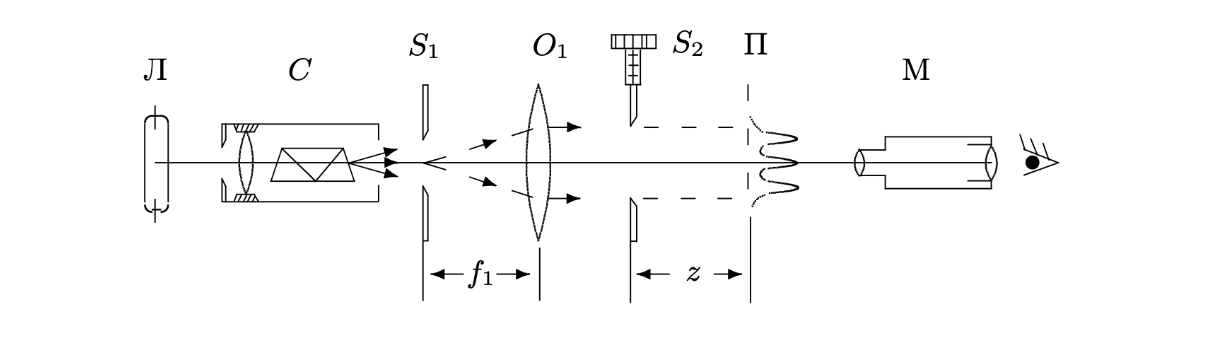
\includegraphics[width=0.8\linewidth]{a.png}
  \caption{Схема установки для наблюдения дифракции Френеля}
  \label{labA}
\end{figure}

Щель $ S_2 $ освещается параллельным пучком монохроматического света с помощью коллиматора, образованного объективом $ O_1 $, и щелью $S_1$, находящейся в его фокусе. На щель $ S_1 $ сфокусировано изображение спектральной линии, выделенной из спектра ртутной лампы Л при помощи простого монохроматора C, в котором используется призма прямого зрения. Распределение интенсивности света в плоскости наблюдения П проще всего рассчитывать с помощью зон Френеля (для щели их иногда называют зонами Шустера). При освещении щели $ S_2 $ параллельным пучком лучей (плоская волна) зоны Френеля представляют собой полоски, параллельные краям щели (рис. \ref{zone}). Результирующая амплитуда в точке наблюдения определяется суперпозицией колебаний от тех зон Френеля, которые не перекрыты створками щели. Графическое определение результирующей амплитуды производится с помощью векторной диаграммы --- спирали Корню. Суммарная ширина $ n $ зон Френеля (Шустера) определяется соотношением:

\begin{equation}\label{xin}
\xi_n = \sqrt{zn\lambda}
\end{equation}
где $ z $ --- расстояние от щели до плоскости наблюдения (рис. \ref{labA}), а $ \lambda $ --- длина волны.

\begin{figure}[h!]
  \centering
  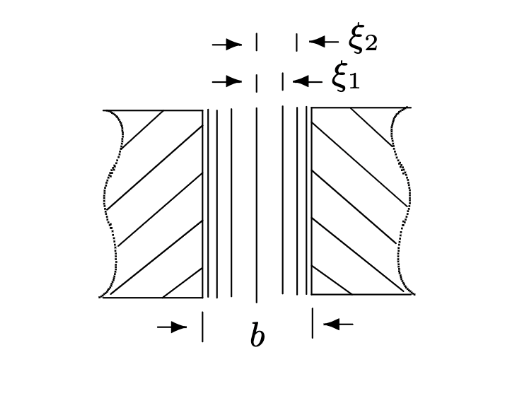
\includegraphics[width=0.3\linewidth]{b.png}
  \caption{Зоны Френеля}
  \label{zone}
\end{figure}

Вид наблюдаемой дифракционной картины
на щели шириной $ b $ определяется волновым параметром $ p $ или числом Френеля $ C $ (число открытых полных зон):


\begin{equation}\label{}
p = \dfrac{\sqrt{z \lambda}}{b}, \qquad C = \dfrac{1}{p^2}
\end{equation}

Дифракционная картина отсутствует вблизи щели при $ p \ll 1 $ ($ C \gg 1 $, т. е. на щели укладывается огромное число зон), а распределение интенсивности света за щелью можно приближённо получить с помощью законов геометрической оптики. Дифракционная картина в этом случае наблюдается только в узкой области на границе света и тени у краёв экрана.

При небольшом удалении от щели (или изменении ширины щели $ S_2 $) эти две группы дифракционных полос перемещаются практически независимо друг от друга. Каждая из этих групп образует картину дифракции Френеля на краю экрана. Распределение интенсивности при дифракции света на краю экрана может быть найдено с помощью спирали Корню.

При дальнейшем увеличении расстояния $ z $ (или уменьшении ширины щели $ S_2 $) обе системы дифракционных полос постепенно сближаются и, наконец, при $ C \gtrsim 1 $ накладываются друг на друга. Распределение интенсивности в плоскости наблюдения в этом случае определяется числом зон Френеля, укладывающихся на полуширине щели $ b/2 $. Если это число равно $ n $, то в поле зрения наблюдается $ m = n - 1 $ тёмных полос. Таким образом, по виду дифракционной картины можно оценить число зон Френеля на полуширине щели.

Параметры установки:
\[ f_1 = 12,5\pm 0,5\;cm \]
\[ f_2 = 12,5\pm 0,5 \;cm \]
\[ \lambda = 5461\;\text{\AA} \]

\subsection{Измерения и обработка результатов}

Найдем нульевое показание микрометрического винта по моменту открытия щели: $l_0 = (0,014 \pm 0,005)$ мм.

Убедимся что свет из щели проходит через все оптические приборы.

Установим линзу \(O_1\) на расстоянии ~ \(F_2 = 12.5\;см\) от \(S_1\). Точно настроим пучок на параллельность с помощью зрительной трубы, собирающей лучи с растаяния в конце коридора.

Ширина щели \(S_2\) -- \(b = 0.33\;мм\), установим ее за линзой \(O_1\).

Установим микроскоп и будем перемещать, получая резкое изображение щели. Видно также что при небольшом удалении микроскопа от щели на ярком фоне изображения щели появляются узкие четкие тёмные полосы.


\begin{table}[H]
  \caption{Зависимость координаты микроскопа от числа $ n $ тёмных полос}
  \label{table1}  
  \begin{center}
    \begin{tabular}{|c|c|c|c|c|c|}
\hline
   \(n\)        &   1  &   2  &   3  &   4  &   5    \\\hline
   \(x_n, cm\)  & 46,6 & 46,2 & 45,9 & 45,7 & 45,6 \\\hline
   \(z_n, cm\)  & 1,3  & 0,9  & 0,6  & 0,4  & 0,3 \\\hline
    \end{tabular}
  \end{center}
\end{table}

Открыв щель \(S_2\) шире и сдвинув микроскоп наблюдаем дифракцию на краю экрана.

Расчитаем зоны Френеля по формуле:
\[ \xi_n = \sqrt{z_nn\lambda} \]

\begin{table}[H]
  \centering
  \begin{tabular}{|c|c|c|c|c|c|}
    \hline
   \(n\)              &  1  & 2   &  3  &  4  &  5    \\\hline
   \(2\xi_n\, мкм\)  & 168 & 198 & 198 & 186 & 181   \\\hline
  \end{tabular}
\end{table}

По полученным данным также построим график зависимости $ 2\xi_n $ от $ n $:

\begin{figure}[H]
  \centering
  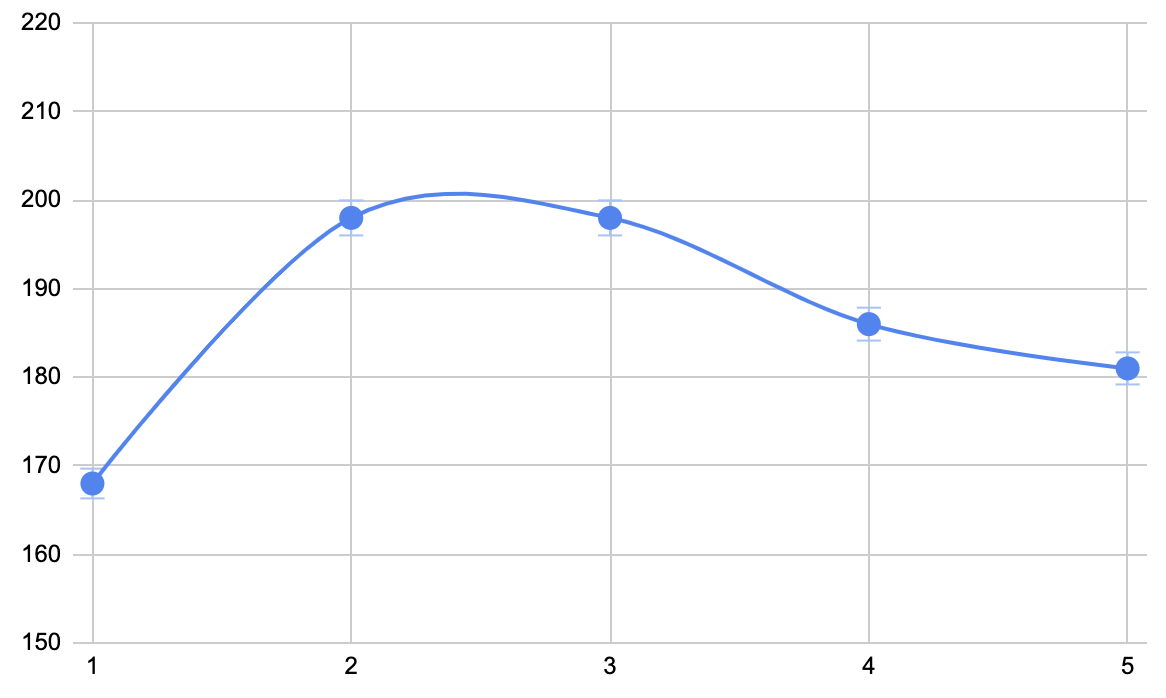
\includegraphics[width=\textwidth]{frnl.png}
\end{figure}



Рассмотрим дифракцию Френеля на препятствии. Поставим вместо щели $ S_2 $ рамку с тонкой вертикальной нитью. При удалении микроскопа можем наблюдать дифракционную картину с характерной светлой полосой на середине препятствия.

\section{Дифракция Фраунгофера на одной щели}

\subsection{Экспериментальная установка}

На значительном удалении от щели, когда выполнено условие $ C \ll 1 $
(то есть ширина щели становится значительно меньше ширины первой
зоны Френеля, $ b \ll \sqrt{\lambda z} $), изображение щели размывается и возникает
дифракционная картина, называемая дифракцией Фраунгофера.

Дифракцию Френеля и Фраунгофера можно наблюдать на одной
и той же установке (рис. \ref{labA}). Однако при обычных размерах установки дифракция Фраунгофера возникает только при очень узких щелях.

\begin{figure}[h!]
  \centering
  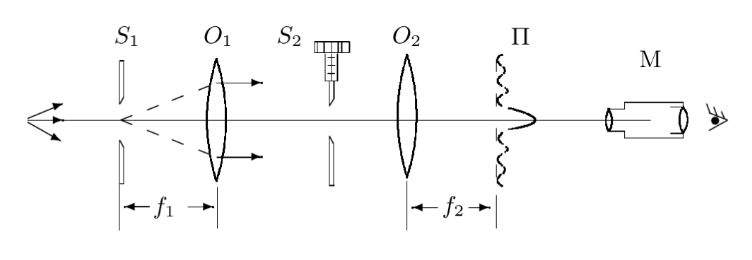
\includegraphics[width=0.8\linewidth]{c.png}
  \caption{Схема установки для наблюдения дифракции Фраунгофера на щели}
  \label{labB}
\end{figure}

Дифракционная картина наблюдается здесь в фокальной плоскости объектива $ O_2 $. Изменением ширины щели добьёмся появления дифракционной картины.

\subsection{Измерения и обработка результатов}

Фокусное расстояние линзы $ f_2 = 12.5$ см.

Координаты \(x_m\) нескольких дифракционных минимумов:

\begin{table}[H]
  \centering
  \begin{tabular}{|c|c|c|c|c|c|}
    \hline
   \(n\)           &  1    & 2     &  3    &  4    &  5    \\\hline
   \(x_n,\;мм\)    & 0,120 & 0,088 & 0,056 & 0,024 & 0 \\\hline
  \end{tabular}
\end{table}


Построим график:
\begin{figure}[H]
  \centering
  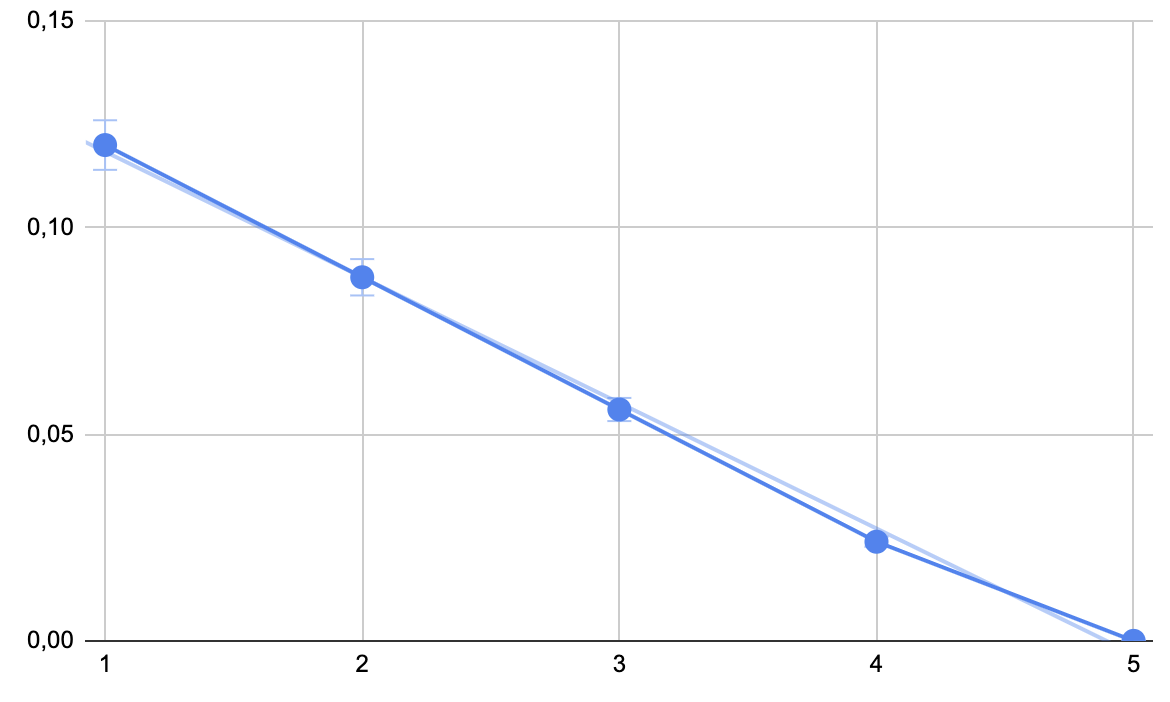
\includegraphics[width=0.8\textwidth]{fgfr.png}
\end{figure}

Полученная зависимость вида \(x_n = (-0.030 \pm 0.005)n + (0.149 \pm 0.005) мм\).

Тогла среднее расстояние \(\Delta x\) между соседними минимумами:
\[ \Delta x = (0.030 \pm 0.001)\; мм \]
Используя формулу:
\[ x_m = m \frac{\lambda}{b}f_2 \]
вычислим значение b:
\[ b = \frac{\lambda f_2}{k} = (2.2 \pm 0.1)\;мм\]

Значение по винту \(b = 0.34\;мм\). Отличие существенное.

\section{Дифракция Фраунгофера на двух щелях}

\subsection{Экспериментальная установка}

Для наблюдения дифракции Фраунгофера на двух щелях в установке (рис. \ref{labB}) следует заменить щель $ S_2 $ экраном Э с двумя щелями
(рис. \ref{labC}). При этом для оценки влияния ширины входной щели на чёткость дифракционной картины вместо входной щели $ S_1 $ следует поставить щель с микрометрическим винтом. Два дифракционных изображения входной щели, одно из которых образовано лучами, прошедшими через левую, а другое --- через правую щели, накладываются друг на друга.

\begin{figure}[h!]
  \centering
  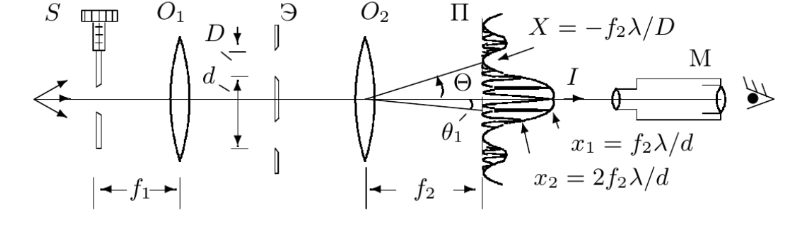
\includegraphics[width=0.8\linewidth]{g.png}
  \caption{Схема установки для наблюдения дифракции Фраунгофера на двух щелях}
  \label{labC}
\end{figure}

\subsection{Измерения и обработка результатов}

C помощью шкалы микроскопа найдем растояние между самыми удалёнными друг от друга тёмными полосами внутри центрального максимума:
\[ l = (0,14 \pm 0,02)\;мм \]

Число светлых промежутков между ними:
\[ N = 8 \]

Расстояние \(\delta x\) между соседними минимумами:
\[ \delta x = \frac{l}{N} = (0,018\pm 0,003)\; мм \]

Расстояние между щелями \(d\) по формуле:
\[ \delta x = f_2\frac{\lambda}{d} \]
Ркзультат вычисления:
\[ d = f_2\frac{\lambda}{\delta x} = (3,8\pm 0,6)\;мм \]

Расстояние между щелями \(d\) с помощью микроскопа:
\[ d = (0,84\pm 0,02)\;мм \]
Значения снова разошлись на порядок, причем повторно.

Увеличивая входную щель, определим её размер при котором наступает первое исчезновение интерференционных полос:
\[ b_0 = (0,08\pm 0,01)\;мм \]

Получим значение \(b_0\) по формуле:
\[ \frac{b_0}{f_1} = \frac{\lambda}{d} \Rightarrow b_0 = f_1\frac{\lambda}{d} = (0,008 \pm 0,002\;мм)\]
Значения вновь разошлись с табличными на порядок.

\section{Вывод и обсуждение результатов}
Мы изучили два основных типа дифракции: Френеля и Фраунгофера при разных размерах щели и провели качественные наблюдения этих явлений, а также экспериментально проверили справедливость теоретических формул.

 Были измерены различные параметры установки:
  \[ b = (2,2 \pm 0,0)\;мм \]
  \[ b_0 = (0,08\pm 0,01)\;мм \]
  \[ d = (3,8\pm 0,6)\;мм \]

 Все эти величины оказались на 1 порядок больше измеренных напрямую. Что наводит на мысль о систематический ошибки в вычислениях или измерениях. Предполагаю, что это было в измерениях, так как в работе тяжело было понять сколько именно интерференционных полос видно и когда они начинают исчезать из-за большой нечеткости изображения. Основной вклад в них могли внести аберрации света, которые могли возникнуть из-за недостаточно точной настройки оптической системы для выполнения работы. Также свой вклад вносит неточность определения линейных размеров объектов при помощи микроскопа, особенно при определении координат дифракционных максимумов.

\end{document}